%=======================================================================%
%
%	DOCUMENT DEFINITION
%
%=======================================================================%

%we use article class because we want to fully customize the page and dont use a cv template
\documentclass[10pt,A4]{article}	

%------------------------------------------------------------------------
%	ENCODING
%------------------------------------------------------------------------
%we use utf8 since we want to build from any machine
\usepackage[utf8]{inputenc}		

%------------------------------------------------------------------------
%	LOGIC
%------------------------------------------------------------------------
% provides \isempty test
\usepackage{xifthen}

%------------------------------------------------------------------------
%	FONT
%------------------------------------------------------------------------
% some tex-live fonts - choose your own
% \usepackage[defaultsans]{droidsans}
% \usepackage[default]{comfortaa}
% \usepackage{cmbright}
% \usepackage[default]{raleway}
% \usepackage{fetamont}
\usepackage[default]{gillius}
% \usepackage[light,math]{iwona}
% \usepackage[thin]{roboto} 

% set font default
\renewcommand*\familydefault{\sfdefault} 	
\usepackage[T1]{fontenc}

% more font size definitions
\usepackage{moresize}		

\usepackage{fontawesome}

%------------------------------------------------------------------------%	PAGE LAYOUT  DEFINITIONS
%------------------------------------------------------------------------

%debug page outer frames
% \usepackage{showframe}			

%define page styles using geometry
\usepackage[a4paper]{geometry}		

% for example, change the margins to 2 inches all round
\geometry{top=1.2cm, bottom=-.6cm, left=0.5cm, right=0.5cm} 	

%less space between header and content
\setlength{\headheight}{-5pt}		

%indentation is zero
\setlength{\parindent}{0mm}

%-----------------------------------------------------------------------
%	TABLE /ARRAY DEFINITIONS
%----------------------------------------------------------------------- 
%for layouting tables
\usepackage{multicol}			
\usepackage{multirow}

%extended aligning of tabular cells
\usepackage{array}

\newcolumntype{x}[1]{%
>{\raggedleft\hspace{0pt}}p{#1}}%

%------------------------------------------------------------------------
%	GRAPHICS DEFINITIONS
%------------------------------------------------------------------------
%for header image
\usepackage{graphicx}

%for floating figures
\usepackage{wrapfig}
\usepackage{float}
%\floatstyle{boxed} 
%\restylefloat{figure}

%for drawing graphics		
\usepackage{tikz}				
\usetikzlibrary{shapes, backgrounds,mindmap, trees}

%------------------------------------------------------------------------
%	Color DEFINITIONS
%------------------------------------------------------------------------
\usepackage{transparent}
\usepackage{color}

%accent color
\definecolor{complcol}{RGB}{250,150,10}

%dark background color
\definecolor{bgcol}{RGB}{110,110,110}

%light background / accent color
\definecolor{softcol}{RGB}{225,225,225}

\definecolor{sectcol}{RGB}{0,120,150}

%Package for links, must be the last package used
\usepackage[colorlinks, urlcolor=blue]{hyperref}

%=======================================================================%
%
%	DEFINITIONS
%
%=======================================================================%

% returns minipage width minus two times \fboxsep
% to keep padding included in width calculations
\newcommand{\mpwidth}{\linewidth-\fboxsep-\fboxsep}
	
%------------------------------------------------------------------------
% 	ARROW GRAPHICS in Tikz
%------------------------------------------------------------------------

% a six pointed arrow poiting to the left
\newcommand{\tzlarrow}{(0,0) -- (0.2,0) -- (0.3,0.2) -- (0.2,0.4) -- (0,0.4) -- (0.1,0.2) -- cycle;}	

% include the left arrow into a tikz picture
% param1: fill color
%
\newcommand{\larrow}[1]
{\begin{tikzpicture}[scale=0.58]
	 \filldraw[fill=#1!100,draw=#1!100!black]  \tzlarrow
 \end{tikzpicture}
}

% a six pointed arrow poiting to the right
\newcommand{\tzrarrow}{ (0,0.2) -- (0.1,0) -- (0.3,0) -- (0.2,0.2) -- (0.3,0.4) -- (0.1,0.4) -- cycle;}

% include the right arrow into a tikz picture
% param1: fill color
\newcommand{\rarrow}
{
\begin{tikzpicture}[scale=0.7]
	\filldraw[fill=sectcol!100,draw=sectcol!100!black] \tzrarrow
 \end{tikzpicture}
}

%------------------------------------------------------------------------
%	custom sections
%------------------------------------------------------------------------

% create a coloured box with arrow and title as cv section headline
% param 1: section title
\newcommand{\cvsection}[1]
{
\colorbox{sectcol}{\mystrut \makebox[1\mpwidth][l]{
\larrow{bgcol} \hspace{-8pt} \larrow{bgcol} \hspace{-8pt} \larrow{bgcol} \textbf{\textcolor{white}{\uppercase{#1}}}\hspace{4pt}
}}\\
}

% create a coloured arrow with title as cv meta section section
% param 1: meta section title
\newenvironment{metasection}[1] {
	\vspace{6pt}
	\begin{center}
		\textcolor{white}{\large{\uppercase{#1}}}\\
	\normalsize
	\parbox{0.7\mpwidth}{\textcolor{white}	\hrule}
}{\end{center}}

%------------------------------------------------------------------------
%	 CV EVENT
%------------------------------------------------------------------------

% creates a stretched box as cv entry headline followed by some paragraphs about 
% the work you did
% param 1:	event time i.e. 2014 or 2011-2014 etc.
% param 2:	event name (what did you do?)
% param 3:	institution (where did you work / study)
% param 4:	list of paragraphs outlining your contributions, see example usage below
\newcommand{\cvevent}[4]
{
\vspace{6pt}
	\begin{tabular*}{1\mpwidth}{p{0.53\mpwidth}  x{0.44\mpwidth}}
 	\textcolor{black}{\textbf{#2}} & \textcolor{complcol}{#3}, \textcolor{bgcol}{#1} 
	\end{tabular*}
\vspace{0pt}
\textcolor{softcol}{\hrule}
\vspace{6pt}
	\cvlist {#4}
\vspace{-6pt}
}

% Same as \cvevent, but without the institution field and more compact
\newcommand{\cvline}[2]
{
\vspace{4pt}
	\begin{tabular*}{1\mpwidth}{p{0.8\mpwidth} x{0.18\mpwidth}}
 	\textcolor{black}{\cvlist {#2}} & \textcolor{bgcol}{	#1} 
	\end{tabular*}
\vspace{0pt}
\textcolor{softcol}{\hrule}
}

% formats a list of strings with variable length for use in `\cvevent`
% param 1: a list of strings outlining your contributions
\newcommand{\cvlist}[1] {
    \foreach \listitem in {#1}
    {
        \begin{tabular*}
            {1\mpwidth}{p{1\mpwidth}}
            \parbox{1\mpwidth}{\larrow{softcol} \listitem}
            \vspace{3pt}
        \end{tabular*}
    }
}

% creates a stretched box as 
\newcommand{\cveventmeta}[2]
{
	\mbox{\mystrut \hspace{87pt}\textit{#1}}\\
	#2
}

%------------------------------------------------------------------------
% CUSTOM STRUT FOR EMPTY BOXES
%----------------------------------------- ------------------------------
\newcommand{\mystrut}{\rule[-.3\baselineskip]{0pt}{\baselineskip}}

% use to vertically center content
% credits to: http://tex.stackexchange.com/questions/7219/how-to-vertically-center-two-images-next-to-each-other
\newcommand{\vcenteredinclude}[1]{\begingroup
\setbox0=\hbox{\includegraphics{#1}}%
\parbox{\wd0}{\box0}\endgroup}

% use to vertically center content
% credits to: http://tex.stackexchange.com/questions/7219/how-to-vertically-center-two-images-next-to-each-other
\newcommand*{\vcenteredhbox}[1]{\begingroup
\setbox0=\hbox{#1}\parbox{\wd0}{\box0}\endgroup}

%------------------------------------------------------------------------
%	ICON-SET EMBEDDING
%------------------------------------------------------------------------

% at this point we simplify our icon-embedding by simply referring to a set of png images.
% if you find a good way of including svg without conflicting with other packages you can
% replace this part
\newcommand{\icon}[3]{\makebox(#2, #2){\textcolor{#3}{\csname fa#1\endcsname}}}	%icon shortcut
\newcommand{\icontext}[4]{ 						%icon with text shortcut
	\vcenteredhbox{\icon{#1}{#2}{#4}} \vcenteredhbox{\textcolor{#4}{#3}}
}
\newcommand{\iconhref}[5]{ 						%icon with website url
    \vcenteredhbox{\icon{#1}{#2}{#5}} \href{#4}{\textcolor{#5}{#3}}
}

\newcommand{\iconemail}[5]{ 						%icon with email link
    \vcenteredhbox{\icon{#1}{#2}{#5}} \href{mailto:#4}{\textcolor{#5}{#3}}
}

\newcommand{\customicon}[3]{
    \newcommand{\tempcmd}{\includegraphics*[width=#2pt, height=#2pt]{#1}} % Create a command
   \makebox(#2, #2){\textcolor{#3}{\tempcmd}}  % Use the command
}   

\newcommand{\customicontext}[4]{ 
   \vcenteredhbox{\customicon{#1}{#2}{#4}} \vcenteredhbox{\textcolor{#4}{#3}}
}

%=======================================================================%
%
%	DOCUMENT CONTENT
%
%=======================================================================%
\begin{document}

%=======================================================================%
%
%	PAGE 1
%
%=======================================================================%
\fcolorbox{white}{white}{\begin{minipage}[c][0.95\textheight][t]{0.77\linewidth}

%=======================================================================%
%	HEADER
%=======================================================================%
%------------------------------------------------------------------------
%	TITLE HEADLINE
%------------------------------------------------------------------------
\vspace{-3pt}
% use this for multiple words like working titles etc.
% \hspace{-0.25\linewidth}\colorbox{bgcol}{\makebox[1.5\linewidth][c]{\hspace{46pt}\HUGE{\textcolor{white}{\uppercase{M.Sc. Jan Küster}} } \textcolor{sectcol}{\rule[-1mm]{1mm}{0.9cm}} \parbox[b]{5cm}{   \large{ \textcolor{white}{{IT Consultant}}}\\
% \large{ \textcolor{white}{{JS Fullstack Engineer}}}}
% }}

% use this for single words, e.g. CV or RESUME etc.
\colorbox{bgcol}{\makebox[\mpwidth][c]{\HUGE{\textcolor{white}{\uppercase{Francesco Ioli}} } \textcolor{sectcol}{\rule[-1mm]{1mm}{0.9cm}} \HUGE{\textcolor{white}{\uppercase{CV}} } }}

%------------------------------------------------------------------------
%	HEADER
%------------------------------------------------------------------------

%\hspace{-1.6cm}
%trimming relative to image size [trim={left bottom right top},clip]
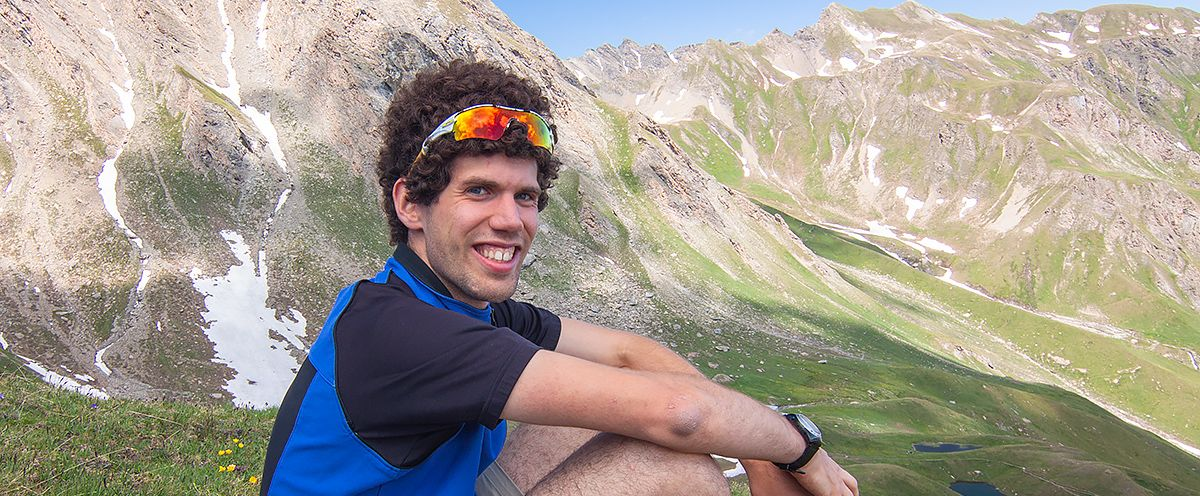
\includegraphics[trim=250 150 0 40, clip,width=\linewidth]{assets/header.jpg}	

\transparent{0.75}%
\vspace{-130pt}
\hspace{0.4\linewidth}
\colorbox{bgcol}{
    \parbox{0.55\linewidth}{
        \transparent{1}
        \begin{center}
            \larrow{sectcol}\larrow{sectcol}
            \textcolor{white}{
                    I hold a PhD in Environmental and Infrastructure Engineering, major in Geoinformatics.\\
                    Specialized in photogrammetry and 3D reconstruction in challenging environments, with a focus on alpine glaciers. \\
                    Skilled in coding and a strong believer in open-source software, data, and science. \\
                    Currently working on deep learning image matching. \\
                    UAV pilot for topographic surveys.
                    }
        \end{center}
    }
}
\vspace{20pt}

%=======================================================================%
%	CV SECTIONS AND EVENTS (MAIN CONTENT)
%=======================================================================%
%-------------------------------------------------------------------------------
%	EDUCATION SECTION
%-------------------------------------------------------------------------------
\cvsection{Education}

\cvevent{2020 - 2024}{PhD (Cum Laude)}{Politecnico di Milano, DICA (IT)}{
\href{https://hdl.handle.net/10589/224092}{PhD Thesis}: \textit{Multi-temporal and Multi-scale photogrammetry for Alpine Glacier Monitoring}.\\
Development of novel photogrammetric techniques for territorial and infrastructural monitoring. 
Created \href{https://github.com/franioli/icepy4d}{ICEpy4D}{,} an image-based pipeline for 4D glacier monitoring with low-cost stereo cameras.  
Contributed to \href{https://github.com/3DOM-FBK/deep-image-matching}{Deep-Image-Matching}{,} a multi-view image matching library with deep learning for SfM.
Application of UAV photogrammetry for structural health assessment{,} including crack detection on concrete bridges.
}

%  My research focuses on photogrammetry and 3D reconstruction for territorial and infrastructural monitoring. 
%  My research focuses on UAV-based and terrestrial photogrammetry for land and infrastructure monitoring. I am working on a low-cost image-based system for 4D glacier monitoring (\href{https://github.com/franioli/icepy4d}{ICEpy4D}) and UAV-photogrammetry for structural health assessment and crack detection on concrete bridges.
%  I am contributing to \href{https://github.com/3DOM-FBK/deep-image-matching}{Deep-Image-Matching]} a multiview matching with deep-learning and hand-crafted local features SfM  
 
 \cvevent{2022}{Visiting PhD student (4 months)}{University of Twente, ITC (NL)}{
Development of a deep learning wide-baseline stereo matching workflow for 4D monitoring of an alpine glacier with low-cost time-lapse cameras. 
\href{https://doi.org/10.1007/s41064-023-00272-w}{[Paper]} \href{https://github.com/franioli/icepy4d}{[Code]}
}

\cvevent{2022}{Innsbruck Summer School of Alpine Research}{Obergurgl (AT)}{
Participation in the Summer School \textit{Close Range Sensing Techniques in Alpine Terrain} \href{https://www.uibk.ac.at/iup/buecher/9783991060819.html}{[Proceedings]}
}


\cvevent{2019 - 2020}{Visiting student for MSc Thesis development}{ETH Zürich, VAW (CH)}{
\textit{Evaluation of Airborne Image Velocimetry approaches with low-cost UAVs in riverine environments}. Supervisors: Prof. Livio Pinto{,} Dr. Martin
Detert \href{http://doi.org/10.13140/RG.2.2.36679.65446}{[Thesis]} \href{https://doi.org/10.5194/isprs-archives-XLIII-B2-2020-597-2020}{[Paper]}
}

\cvevent{2017 - 2020}{MSc Environmental and Land Planning Engineering}{Politecnico di Milano}{Major in Land Monitoring and Diagnostics. Grade 110L/110.
}

\cvevent{2019}{Erasmus Exchange}{Aalto University, Helsinki (FIN)}{}

\cvevent{2014 - 2017}{BSc Environmental and Land Planning Engineering}{Politecnico di Milano}{
BSc	Thesis: \textit{Snowpack surveys aimed at hydrological analysis: a case study carried out with UAVs and manual probing measurements on the Belvedere glacier (Macugnaga, Italian Alps)}. Grade 102/110.
}

\vspace{6pt}
\begin{tabular*}{1\mpwidth}{p{0.48\mpwidth}  x{0.50\mpwidth}}
\textcolor{black}{\textbf{Scientific High School}} & \textcolor{complcol}{Liceo Scientifico Falcone e Borsellino}, \textcolor{bgcol}{2009 - 2013} 
\end{tabular*}
\textcolor{softcol}{\hrule}


\vspace{12pt}

%------------------------------------------------------------------------
%	EXPERIENCE
%------------------------------------------------------------------------

\cvsection{Experience}
% \vspace{-2pt}

\cvevent{2020 - now}{Teaching Assistant}{Politecnico di Milano}{
\textit{Trattamento delle Osservazini} - Statistics (BSc) [2020 - 2021 - 2022 - 2023],
\textit{Sistemi Informativi Territoriali} - GIS (BSc) [2020 - 2021],
\textit{Tecniche di rilievo e modellazione 3D per l'architettura} - 3D modelling for architecture (BSc) [2020 - 2021 - 2022].
}

\cvevent{2021 - 2024}{Tutoring in Summer School}{Politecnico di Milano}{\textit{Design and Execution of Topographic Surveys for Land Monitoring} @ Belvedere Glacier (IT) aimed at introducing BSc and MSc students to topographic fieldwork in mountain environments. 
}

\cvevent{2022}{Topographic technical consultant}{Prof. Alberto Bianchi}{Topographic consultant for the Technical Consultant of Office and Part (CTU) R.G. 717/2019}

\cvevent{2022}{Topographic technician}{Gini Telecom}{UAV surveys for telecommunication antennas}
\vspace{12pt}

% \textcolor{softcol}{\hrule}

\end{minipage}}% DO NOT LEAVE A BLANK LINE HERE!
%=======================================================================%
%	METADATA
%=======================================================================%
\fcolorbox{white}{sectcol}{\begin{minipage}[c][0.95\textheight][t]{0.20\linewidth}
    \begin{metasection}{Contact}

    \icontext{MapMarker}{12}{Milano, Italy}{white}\\[4pt]
    \icontext{Male}{12}{03/09/1995}{white}\\[4pt]
    \iconemail{Send}{12}{\small francesco.ioli@polimi.it}{francesco.ioli@polimi.it}{white}\\[4pt]
    \iconhref{Globe}{12}{franioli.github.io}{https://franioli.github.io}{white}\\[4pt]
    \iconhref{Linkedin}{12}{francesco-ioli}{https://www.linkedin.com/in/francesco-ioli-640061160/}{white}\\[4pt]
    \iconhref{Github}{12}{github.com/franioli}{https://github.com/franioli}{white}\\[4pt]
    \iconhref{Twitter}{12}{@francescoioli}{https://twitter.com/francescoioli}{white}\\[4pt]
    \iconhref{GraduationCap}{12}{Scholar: Francesco Ioli}{https://scholar.google.com/citations?user=hZkC2UMAAAAJ}{white}\\[4pt]
    \iconhref{LineChart}{12}{H-Index (Scopus): 6}{https://www.scopus.com/authid/detail.uri?authorId=57219022961}{white}\\[4pt]
\end{metasection}

\begin{metasection}{Programming}

\textcolor{white}{
    \icontext{Code}{12}{Python}{white}\icon{Star}{8}{complcol}\icon{Star}{8}{complcol}\icon{Star}{8}{complcol}\icon{Star}{8}{complcol}\\[4pt]
    \icontext{Code}{12}{Matlab}{white}\icon{Star}{8}{complcol}\icon{Star}{8}{complcol}\icon{Star}{8}{white}\icon{Star}{8}{white} \\[4pt]
    \icontext{Code}{12}{C++}{white} \icon{Star}{8}{complcol}\icon{Star}{8}{white}\icon{Star}{8}{white}\icon{Star}{8}{white}  \\[4pt]
    }
\end{metasection}

\begin{metasection}{Photogrammetry}

\textcolor{white}{
    \customicontext{assets/metashape}{10}{Agisoft Metashape}{white} \\[2pt]
    \customicontext{assets/photomodeler}{10}{Photomodeler}{white} \\[2pt]
    \customicontext{assets/cloudcompare}{10}{CloudCompare}{white} \\[2pt]
    \customicontext{assets/icon_pcd}{10}{COLMAP MicMac}{white} \\[2pt]
    \customicontext{assets/logo_odm}{10}{OpenMVG ODM}{white} \\[2pt]
    }
\end{metasection}

\begin{metasection}{Tools}

\textcolor{white}{
    \customicontext{assets/pytorch}{10}{Pytorch}{white}\\[2pt]
    \icontext{Database}{10}{PostgreSQL PostGis}{white} \\[2pt]
    \customicontext{assets/docker}{10}{Docker}{white}\\[2pt]
    \icontext{Gears}{10}{Raspberry Arduino}{white} \\ [2pt]
    \icontext{CodeFork}{10}{Git}{white} \\[2pt]
    \icontext{FileTextO}{10}{Latex}{white} \\[2pt]
    }
\end{metasection}

\begin{metasection}{Other software}

\textcolor{white}{
    \icontext{MapO}{10}{QGIS ESRI ArcGIS}{white} \\[2pt]
    \icontext{Globe}{10}{Rtklib Leica Infinity}{white} \\[2pt]
    \icontext{PaintBrush}{10}{Photoshop Lightrooom}{white} \\[2pt]
    \icontext{PaintBrush}{10}{GIMP Inkscape}{white} \\[2pt]
    \icontext{PencilSquareO}{10}{AutoCAD}{white} \\[2pt]
    }
\end{metasection}

\begin{metasection}{Operating Systems}

\textcolor{white}{
    \Large \icon{Linux}{20}{white} \Large \icon{Windows}{20}{white}
    }
\end{metasection}

\begin{metasection}{Hobbies}

\textcolor{white}{
    \customicon{assets/mountain}{20}{white}
    \icon{Camera}{18}{white} 
    \icon{Bicycle}{18}{white}
    }
\end{metasection}

%-------------------------------------------------------------------------------
%	QR CODE (optional)
%-------------------------------------------------------------------------------
% \vspace{12pt}
% \begin{center}
% \includegraphics[width=0.35\mpwidth]{assets/qrcode}
% \end{center}

\end{minipage}}

%------------------------------------------------------------------------
% FOOTER (footer cannot exceed linewidth) 
%------------------------------------------------------------------------

\null
\vspace*{\fill}
\hspace{-0.25\linewidth}\colorbox{bgcol}{\makebox[1.5\linewidth][c]{\mystrut \small \textcolor{white}{Francesco Ioli - \today}}}\\[-6pt]

%=======================================================================%
%
%	PAGE 2
%
%=======================================================================%
\newpage

\cvsection{Selected pubblications}

\cvlist{\underline{Ioli{,} F.}{,} Dematteis{,} N.{,} Giordan{,} D.{,} 
Nex{,} F. Pinto{,} L.{,} 2024. Deep Learning Low-cost Photogrammetry for 4D Short-term Glacier Dynamics Monitoring. \textit{PFG – Journal of Photogrammetry, Remote Sensing and Geoinformation Science} \href{https://doi.org/10.1007/s41064-023-00272-w}{[Paper]} \href{https://github.com/franioli/icepy4d}{[Code]}}

\cvlist{
\underline{Ioli{,} F.}{,} De Gaetani{,} C.{,} Barbieri{,} F.{,} Gaspari{,} F.{,} Pinto{,} L.{,} Rossi{,} L.{,} 2024. Belvedere Glacier long-term monitoring Open Data (2.0) [Data set]. Zenodo. \href{https://doi.org/10.5281/zenodo.10817029}{[Dataset]} \href{https://thebelvedereglacier.it/}{[Web-app]}
}

\cvlist{
Morelli{,} L.{,} \underline{Ioli{,} F.}{,} Maiwald{,} F.{,} Mazzacca{,} G.{,} Menna{,} F.{,} Remondino{,} F.{,} 2024. Deep-Image-Matching: a Toolbox for Multi-view Image Matching of Complex Scenarios. \textit{Int. Arch. Photogramm. Remote Sens. Spatial Inf. Sci.}{,} XLVIII-2/W4-2024{,} 309–316 \href{https://doi.org/10.5194/isprs-archives-XLVIII-2-W4-2024-309-2024}{[Paper]} \href{https://github.com/3DOM-FBK/deep-image-matching}{[Code]}
}

\cvlist{
Gaspari{,} F.{,} Barbieri{,} F.{,} Fascia{,} R.{,} \underline{Ioli{,} F.}{,} Pinto{,} L.{,} 2024. An Open-Source Web Platform for 3D Documentation and Storytelling of Hidden Cultural Heritage. \textit{Heritage} 7(2){,} 517-536 \href{https://doi.org/10.3390/heritage7020025}{[Paper]} \href{https://github.com/labmgf-polimi/potree-chtemplate}{[Code]}
\href{https://labmgf.dica.polimi.it/pujob/potree-template/}{[Web-app]}
}

\cvlist{Gaspari{,} F.{,} \underline{Ioli{,} F.}{,} Barbieri{,} F.{,} Bonora{,} S.{,} Fascia{,} R.{,} Pinto{,} L.{,} Migliaccio{,} F.{,} 2024. Bridging geomatics theory to real-world applications in alpine surveys through an innovative summer school teaching program. \textit{Int. Arch. Photogramm. Remote Sens. Spatial Inf. Sci.{,}} XLVIII-4/W12-2024{,} 59–66{,} \href{https://doi.org/10.5194/isprs-archives-XLVIII-4-W12-2024-59-2024}{[Paper]}}

\cvlist{
Morelli{,} L.{,} Mazzacca{,} G.{,} Trybała{,} P.{,} Gaspari{,} F.{,} \underline{Ioli{,} F.}{,} Ma{,} Z.{,} Remondino{,} F.{,} Challis{,} K.{,} Poad{,} A.{,} Turner{,} A.{,} and Mills{,} J. P.{,} 2024. The Legacy of Sycamore Gap: The Potential of Photogrammetric AI for Reverse Engineering Lost Heritage with Crowdsourced Data. \textit{Int. Arch. Photogramm. Remote Sens. Spatial Inf. Sci.}{,} XLVIII-2-2024{,} 281–288{,} \href{https://doi.org/10.5194/isprs-archives-XLVIII-2-2024-281-2024}{[Paper]} \href{http://137.117.39.162:10088/}{[Web-app]}
}

\cvlist{
\underline{Ioli{,} F.}{,} Bruno{,} E.{,} Calzolari{,} D.{,} Galbiati{,} M.{,} Mannocchi{,} A.{,} Manzoni{,} P.{,} Martini{,} M.{,} Bianchi{,} A.{,} Cina{,} A.{,} De Michele{,} C.{,} and Pinto{,} L.{,} 2023. A REPLICABLE OPEN-SOURCE MULTI-CAMERA SYSTEM FOR LOW-COST 4D GLACIER MONITORING{,} \textit{Int. Arch. Photogramm. Remote Sens. Spatial Inf. Sci.}{,} XLVIII-M-1-2023{,} 137–144{,} \href{https://doi.org/10.5194/isprs-archives-XLVIII-M-1-2023-137-2023}{[Paper]}
}

\cvlist{
Morelli{,} L.{,} \underline{Ioli{,} F.}{,} Beber{,} R.{,} Menna{,} et al.{,} 2023. COLMAP-SLAM: a Framework for Visual Odometry{,} \textit{Int. Arch. Photogramm. Remote Sens. Spatial Inf. Sci.}{,} XLVIII-1/W1-2023{,} 317–324 \href{https://doi.org/10.5194/isprs-archives-XLVIII-1-W1-2023-317-202}{[Paper]} \href{https://github.com/3DOM-FBK/COLMAP_SLAM}{[Code]}
}

\cvlist{
\underline{Ioli{,} F.}{,} Barbieri{,} F.{,} Gaspari{,} F.{,} Nex{,} F.{,} and Pinto{,} L.{,} 2023. ICEPY4D: A PYTHON TOOLKIT FOR ADVANCED MULTI-EPOCH GLACIER MONITORING WITH DEEP-LEARNING PHOTOGRAMMETRY{,} \textit{Int. Arch. Photogramm. Remote Sens. Spatial Inf. Sci.}{,} XLVIII-1/W2-2023{,} 1037–1044{,} \href{https://doi.org/10.5194/isprs-archives-XLVIII-1-W2-2023-1037-2023}{[Paper]} \href{https://github.com/franioli/icepy4d}{[Code]}
}

\cvlist{
Gaspari{,} F.{,} Barbieri{,} F.{,} Duque{,} J. P.{,} Fascia{,} R.{,} \underline{Ioli{,} F.}{,} Zani{,} G.{,} Carrion{,} D.{,} and Pinto{,} L.{,} 2023. A GEO-DATABASE FOR 3D-AIDED MULTI-EPOCH DOCUMENTATION OF BRIDGE INSPECTIONS{,} \textit{Int. Arch. Photogramm. Remote Sens. Spatial Inf. Sci.}{,} XLVIII-1/W2-2023{,} 299–306{,} \href{https://doi.org/10.5194/isprs-archives-XLVIII-1-W2-2023-299-2023}{[Paper]}
}

\cvlist{
Gaspari{,} F.{,} Barbieri{,} F.{,} Demnati{,} I.{,} \underline{Ioli{,} F.}{,} Pinto{,} L.{,} and Toscani{,} V.{,} 2023. MOBILE MAPPING SOLUTIONS FOR THE UPDATE AND MANAGEMENT OF TRAFFIC SIGNS IN A ROAD CADASTRE FREE OPEN-SOURCE GIS ARCHITECTURE{,} \textit{Int. Arch. Photogramm. Remote Sens. Spatial Inf. Sci.}{,} XLVIII-4/W7-2023{,} 61–66{,} \href{https://doi.org/10.5194/isprs-archives-XLVIII-4-W7-2023-61-2023}{[Paper]}
}

\cvlist{
\underline{Ioli{,} F.}{,} Bianchi{,} A.{,} Cina{,} A.{,} De Michele{,} et al.{,} 2022. Mid-Term Monitoring of Glacier’s Variations with  UAVs: The Example of the Belvedere Glacier. \textit{Remote Sensing} 14{,} 28 \href{https://doi.org/10.3390/rs14010028}{[Paper]} \href{https://zenodo.org/doi/10.5281/zenodo.7842347}{[Open Data]} \href{https://thebelvedereglacier.it/}{[Web Platform]}
}


\cvlist{
\underline{Ioli{,} F.}{,} Pinto{,} A.{,} Pinto{,} L.{,} 2022. UAV-Photogrammetry for Metric Evaluation of Concrete Bridge Cracks. \textit{Int. Arch. Photogramm. Remote Sens. Spatial Inf. Sci.} XLIII-B2-2022{,} 1025–1032 \href{https://doi.org/10.5194/isprs-archives-XLIII-B2-2022-1025-2022}{[Paper]} \href{https://github.com/franioli/Cracks}{[Code]}
}

\cvlist{
Gaspari{,} F.{,} \underline{Ioli{,} F.}{,} Barbieri{,} F.{,} Belcore{,} E.{,} and Pinto{,} L.{,} 2022. INTEGRATION OF UAV-LIDAR AND UAV-PHOTOGRAMMETRY FOR INFRASTRUCTURE MONITORING AND BRIDGE ASSESSMENT{,} \textit{Int. Arch. Photogramm. Remote Sens. Spatial Inf. Sci.}{,} XLIII-B2-2022{,} 995–1002{,} \href{https://doi.org/10.5194/isprs-archives-XLIII-B2-2022-995-2022}{[Paper]}
}

\cvlist{
De Gaetani{,} C.I.{,} \underline{Ioli{,} F.}{,} Pinto{,} L.{,} 2021. Aerial and UAV Images for Photogrammetric Analysis of Belvedere Glacier Evolution in the Period 1977–2019 \textit{Remote Sensing} 13{,} 3787. \href{https://doi.org/10.3390/rs13183787}{[Paper]}
}

\cvlist{
Rossi{,} L.{,} \underline{Ioli{,} F.}{,} Capizzi{,} E.{,} Pinto{,} L.{,} and Reguzzoni{,} M.{,} 2021. IMPROVING UAV TELEMETRY POSITIONING FOR DIRECT PHOTOGRAMMETRY{,} \textit{Int. Arch. Photogramm. Remote Sens. Spatial Inf. Sci.}{,} XLIII-B2-2021{,} 61–68{,} \href{https://doi.org/10.5194/isprs-archives-XLIII-B2-2021-61-2021}{[Paper]}
}

\cvlist{
\underline{Ioli{,} F.}{,} Pinto{,} L.{,} Passoni{,} D.{,} Nova{,} V.{,} Detert{,} M.{,} 2020. Evaluation of Airborne Image Velocimetry approaches using low-cost UAVs in riverine Environments. \textit{Int. Arch. Photogramm. Remote Sens. Spatial Inf. Sci.} Vol.XLIII-B2-2020{,} 597–604 \href{https://doi.org/10.5194/isprs-archives-XLIII-B2-2020-597-2020}{[Paper]}
} \vspace{12pt}

\cvsection{Presentations in scientific conferences}

\cvlist{2024: EGU - Wien (oral) \href{https://meetingorganizer.copernicus.org/EGU24/EGU24-16412.html}{[Abstract]}
}

\cvlist{2023: EGU - Wien (oral) \href{https://meetingorganizer.copernicus.org/EGU23/EGU23-10018.html}{[Abstract]}{,} ISPRS Geospatial Week - Cairo (oral) \href{https://doi.org/10.5194/isprs-archives-XLVIII-1-W2-2023-1037-2023}{[Paper]}{,} VGC Dresden (oral) \href{https://doi.org/10.25368/2023.194}{[Proceedings]}{,} SIFET congress - Arezzo (IT) (oral) \href{https://www.sifet.org/convengo-2023}{[Link]}{,}  GeoAI - Torino (IT) (oral) \href{https://sites.google.com/view/geo-ai-2023/home}{[Link]}
}

\cvlist{2022: EGU - Wien (oral) \href{https://meetingorganizer.copernicus.org/EGU22/EGU22-7967.html}{[Abstract]}{,} ISPRS Congress - Nice (poster) \href{https://doi.org/10.5194/isprs-archives-XLIII-B2-2022-1025-2022}{[Paper]}
}



 \vspace{12pt}

\cvsection{Contributions to Open Source Software and Data}

\cvlist{\textit{Deep-Image-Matching}: Multiview matching with deep-learning and hand-crafted local features for COLMAP and other SfM software \href{https://github.com/3DOM-FBK/deep-image-matching}{[github.com/3DOM-FBK/deep-image-matching]}}

\cvlist{\textit{Belvedere Glacier Open Data}: web platform for exploring 3D photogammetric point cloud and download data \href{https://thebelvedereglacier.it}{[thebelvedereglacier.it]}
\href{https://zenodo.org/doi/10.5281/zenodo.7842347}{[doi.org/10.5281/zenodo.7842347]}
}

\cvlist{\textit{ICEpy4D}: a multi-purpose Python package for 4D image-based continuous monitoring of glacier evolution using with deep learning SfM and low-cost stereo-cameras \href{https://github.com/franioli/icepy4d}{[github.com/franioli/icepy4d]}}

\cvlist{\textit{COLMAP SLAM}: visual-SLAM based on COLMAP API~\href{https://github.com/3DOM-FBK/COLMAP_SLAM/}{[github.com/3DOM-FBK/COLMAP\_SLAM]} }

\cvlist{\textit{Metashapelib}: a toolbox for extending capabilities of Agisoft Metashape and performing Monte Carlo simulations \href{https://github.com/franioli/metashapelib/}{[github.com/franioli/metashapelib]}} \vspace{12pt}

\cvsection{Grants and awards}

\cvlist{Awarded for the Open Data Day 2024 \href{https://blog.okfn.org/2024/02/28/and-the-winners-of-the-open-data-day-2024-mini-grants-are/}{Mini-grant} from \href{https://blog.okfn.org/}{Open Knowledge Fundation} for the organization of the webinar \href{https://labmgf.dica.polimi.it/opendataday/}{Mapping Climate Change in 4D: Belvedere Glacier’s Open Geo Data for Education and Research}. \href{https://blog.okfn.org/2024/03/28/oddstories-2024-milan-italy/}{[Event Report]}
}

\cvlist{First prize in the 
\href{https://www.dica.polimi.it/francesco-ioli-primo-classificato-nel-premio-giovani-2023-sezione-ricerca/}{Young Researcher Prize} of the Italian Society of Photogrammetry and Remote Sensing (SIFET) 2023
}

\cvlist{Winner of the \href{https://www.egu.eu/education/teg/hetg/2023/}{EGU Higher Education Teaching Grant} for the open teaching material for the Summer School "Design and implementation of topographic surveys for territorial monitoring in mountain environments" \href{https://tars4815.github.io/belvedere-summer-school/}{[Teaching material]}.}

\cvlist{Finalist in the EGU2024 Photo Competition [\href{https://blogs.egu.eu/geolog/2024/04/08/egu24-photo-competition-finalists-who-will-you-vote-for/}{Link}]} \vspace{12pt}

\cvsection{Thesis supervision}

\cvlist{2023/2024: Luca Cerina{,} Very-High Resolution Satellite Stereo Images for Alpine Glacier Monitoring. MSc Course in Environmental and Land Planning Engineering. Supervisor: prof. Livio Pinto.
}

\cvlist{2023/2024: Samuele Bonora{,} Progettazione e implementazione di un database georeferenziato per il monitoraggio del Ghiacciaio del Belvedere. MSc Course in Environmental and Land Planning Engineering. Supervisor: prof. Federica Migliaccio.
}

\cvlist{2021/2022: Irene Pincolini{,} Digital Image Correlation for ice flow velocity estimation: a case study on the Belvedere Glacier with UAV orthophotos. MSc Course in Environmental and Land Planning Engineering. Supervisor: prof. Livio Pinto.
}

\cvlist{2020/2021: Federico Barbieri{,} Monitoraggio Di Aree Alpine Inaccessibili Con Fotogrammetria UAV Low-Cost. MSc Course in Environmental and Land Planning Engineering. Supervisor: prof. Livio Pinto.
}

\cvlist{2020/2021: Pinto Alessandro{,} Tecniche fotogrammetriche da drone per la ricostruzione metrica di fessure su ponti in calcestruzzo. MSc Course in Environmental and Land Planning Engineering. Supervisor: prof. Livio Pinto.
}

\cvlist{2019/2020: Francesco Ferrario{,} Triangolazione Aerea Assistita da DGPS In Fotogrammetria Da Uav: Sperimentazione Di Una Soluzione A Basso Costo Per Il Dji Matrice 210 V2. MSc Course in Environmental and Land Planning Engineering. Supervisor: prof. Livio Pinto.
} \vspace{12pt}

\cvsection{Additional Information}

\cvlist{Languages: Italian (Mother tongue){,} English (C1 - IELTS Certificate 2019)}

\cvlist{UAS License: EASA A2 Open Category{,} with Critical Scenario License}

\cvlist{Driver's license: B}

\cvlist{Professional qualification: \textit{Esame di Stato} for civil and environmental engineers}

\cvlist{Volunteer Experience: \\ \vspace{3pt}
\hspace*{3pt}\begin{tabular}{l l}
    \textit{Apwoyo} (association for homeless people support) & [2023 - now]\\
    Scout Chief in the Italian Scout Association \textit{AGESCI} &[2017 - 2023]\\ 
    Operazione Mato Grosso (charity organization) & [2016 - 2017] \\
    Libera. Associazioni{,} Nomi e Numeri contro le mafie (Anti-mafia association) & [2012 - 2016] \\
\end{tabular}
} \vspace{12pt}


%------------------------------------------------------------------------
% FOOTER (footer cannot exceed linewidth) 
%------------------------------------------------------------------------

% \null
% \vspace*{\fill}
% \hspace{-0.25\linewidth}\colorbox{bgcol}{\makebox[1.5\linewidth][c]{\mystrut \small \textcolor{white}{Francesco Ioli - \today}}}\\[-6pt]

%=======================================================================%
%
%	PAGE 2
%
%=======================================================================%
% \newpage



%------------------------------------------------------------------------
% Closing
%------------------------------------------------------------------------
\null
\vspace*{\fill}
\begin{center}
    \textit{\small According to Regulation of the European Parliament 679/2016, I hereby express my consent to process and use my data in this CV and application for recruiting purposes.}
\end{center}

%------------------------------------------------------------------------
% FOOTER (footer cannot exceed linewidth) 
%------------------------------------------------------------------------
\null
\hspace{-0.25\linewidth}\colorbox{bgcol}{\makebox[1.5\linewidth][c]{\mystrut \small \textcolor{white}{Francesco Ioli - \today}}}\\[-6pt]

%=======================================================================%
%
%	DOCUMENT END
%
%=======================================================================%
\end{document}